\documentclass{article}
\usepackage{graphicx} % Required for inserting images
\usepackage[utf8]{inputenc}
\usepackage{amsmath}
\usepackage{graphicx}
\usepackage{tikz}
\usepackage{array}
\usetikzlibrary{trees}
\usepackage{amssymb}
\usepackage{amsthm}
\usepackage{multirow}
\usepackage{dcolumn}
\usepackage{verbatim}
\usepackage{booktabs}

\newcolumntype{2}{D{.}{}{2.0}}

\title{CSC279 HW5}
\author{Hanzhang Yin}
\date{Nov/13/2023}

\begin{document}

\maketitle

\subsection*{Collaborator}
Chenxi Xu, Yekai Pan, Yiling Zou, Boyi Zhang

\subsection*{PROBLEM 15}
\\
\textbf{Answer: }

\begin{enumerate}
    \item Assume $q$ is inside $P$. We want to find the closest point to $q$ in $\{p_1, \dots, p_n\}$.
    \\
    \textbf{Reasoning: }
    \\
    Hard and required $\Omega(n)$ runtime. Arrange all points on the circumference of a circle like regular convex n-polygon enclosing point $q$ as its center. 
    If the algorithm is deterministic and assumes an easy case, some points remain unvisited. For those unvisited point, we one of them closer.
    Therefore, the algorithm can not find the correct closest point and outputting incorrect results.
    \item Assume $q$ is outside $P$. We want to find the closest point to $q$ in $\{p_1, \dots, p_n\}$.
    \\
    \textbf{Reasoning: }
    \\
    Hard and required $\Omega(n)$ runtime. Place all points on a quarter-circle like regular convex n-polygon enclosing point $q$ while ensuring $P$ is convex and non-enclosing.
    Assume easy, then there will be some point that the algorithm (deterministic) will not visit. For an unvisited point, we move it closer. 
    Therefore, the algorithm can not find the correct closest point and outputting incorrect results.
    \item Assume $q$ is inside $P$. We want to find the farthest point to $q$ in $\{p_1, \dots, p_n\}$.
    \\
    \textbf{Reasoning: }
    \\
    Hard and required $\Omega(n)$ runtime. Similar to Q1, but this time we move an unvisited point further.
    \item Assume $q$ is outside $P$. We want to find the farthest point to $q$ in $\{p_1, \dots, p_n\}$.
    \\
    \textbf{Reasoning: }
    \\
    Hard and required $\Omega(n)$ runtime. Similar to Q2, but this time we move an unvisited point further.
    \item Assume $q$ is inside $P$. We want to find the closest point to $q$ on $P$.
    \\
    \textbf{Reasoning: }
    \\
    Hard and required $\Omega(n)$ runtime. Similar to Q1 again, The number of edges equals the number of points, so we still need at least $O(n)$ runtime.
    \item Assume $q$ is outside $P$. We want to find the closest point to $q$ on $P$.
    \\
    \textbf{Reasoning: }
    \\
    Easy and can be solved within $O(logn)$. 
    \\
    The algorithm finds the closest point to \( q \) on a convex polygon \( P \) in \( O(\log n) \) time using the unimodal nature of the distance function from \( q \) to \( P \). 
    Using ternary search on the edges of \( P \), it narrows the search interval until the closest edge is identified, and then computes the closest point on that edge. 
    The convexity of \( P \) ensures the unimodal property, guaranteeing the correctness of the ternary search.
    
    \begin{verbatim}
        def closest_point_on_convex_polygon(q, P):
            n = len(P)
            low = 0
            high = n - 1

        while high - low > 3:
            m1 = low + (high - low) // 3
            m2 = high - (high - low) // 3

            D_m1 = distance_to_edge(q, P[m1], P[(m1 + 1) % n])
            D_m2 = distance_to_edge(q, P[m2], P[(m2 + 1) % n])

            if D_m1 < D_m2:
                high = m2
            else:
                low = m1

        min_dist = float('inf')
        closest_point = None

        for i in range(low, high + 1):
            p1 = P[i]
            p2 = P[(i + 1) % n]
            c = closest_point_on_segment(q, p1, p2)
            D = distance(q, c)
            if D < min_dist:
                min_dist = D
                closest_point = c

        return closest_point
    \end{verbatim}
    \item Assume $q$ is inside $P$. We want to find the farthest point to $q$ on $P$.
    \\
    \textbf{Reasoning: }
    \\
    Hard and required $\Omega(n)$ runtime. Similar to Q3, so similar argument can be made.
    \item Assume $q$ is outside $P$. We want to find the farthest point to $q$ on $P$.
    \\
    \textbf{Reasoning: }
    \\
    Hard and required $\Omega(n)$ runtime. Similar to Q4. The farthest point must lie on the circumcircle as all other points are on an n-gon, so similar argument can be made.
\end{enumerate}

\newpage

\subsection*{PROBLEM 16}

\begin{figure*}[h]
    \centering
    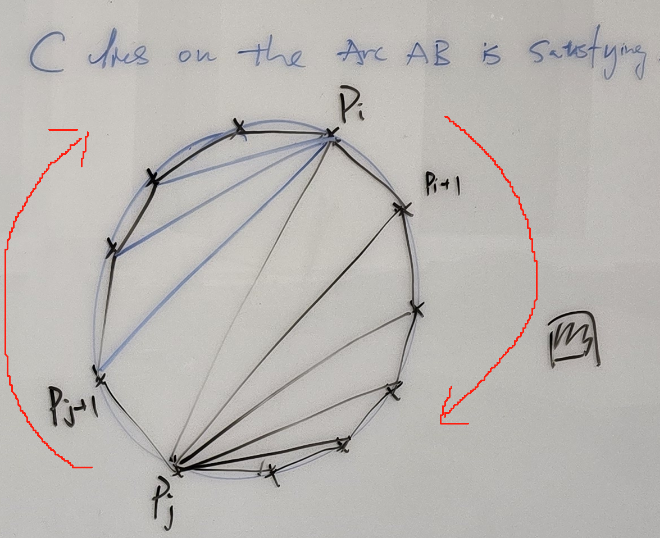
\includegraphics[width=0.7\textwidth]{HW5_Q2.png}
    \label{fig:q2PROOF}
\end{figure*}

\begin{proof}
    Let $\{P_1, \dots, P_n\}$ be the collection of points of a convex polygon $P$.
    \\
    \textbf{Steps for Triangulation: }

    \begin{enumerate}
        \item Order points in clock-wise order $\{p_1, ..., p_n\}$.

        \item Pick the \textbf{longest side} from \textbf{diagonal} or \textbf{side} of $P$: $P_i, P_j$.

        \item Pick the third point $P_k$ such that $P_k$ is the neighbor of point $p_i$ OR $p_j$. WLOG, 
        pick the neighbor of $p_i$ as the third point. We denote the third point as $P_{i+1}$ or $P_{j-1}$.
        \textbf{Note:} This $P_k$ is on the opposite arc from $P_i P_j$.
        \item Form the first triangle as $\triangle P_i P_j P_k$:
        \begin{enumerate}
            \item Then we iteratively add the rest of the polygon of the ``half'' of the polygon as:
            \\
            \textbf{Note:} The neighbor of $P_{i + n}$ is $P_{j - 1}$ and $P_{j - 3}$.
            \[
                P_j P_{j+1} P_{j+2}, \dots, P_{j} P_{i + n} P_{j-1}
            \]

            \item For the rest of the ``half'' of the polygon:
            \\
            \textbf{Note:} The neighbor of $P_{j + m}$ is $P_{i - 1}$ and $P_{i - 3}$.
            \[
                P_i P_j P_{j+1}, \dots, \dots, P_{i} P_{j + m} P_{i-1}.
            \]
        \end{enumerate}
\end{enumerate}

\end{proof}

\subsection*{PROBLEM 17}
The algorithm identifies all "good" points by first constructing the Voronoi diagram of the given points, which efficiently captures proximity relationships in \( O(n \log n) \) time. 
For each point \( p_i \), it examines only its neighboring points in the Voronoi diagram, as these are the only ones that could potentially interfere with placing a new circle. By computing the angular intervals where a circle of radius \( \ell \) touching \( C_i \) would intersect any neighboring \( C_j \), 
the algorithm determines the directions that are blocked. If there exists at least one direction where such interference does not occur, the point \( p_i \) is therefore "good".

\begin{verbatim}
# Helper Functions
def compute_interfering_angles(p_i, p_j, r, l, d_ij):
    # Calculate the angle between p_i and p_j
    delta_x = p_j.x - p_i.x
    delta_y = p_j.y - p_i.y
    alpha = atan2(delta_y, delta_x)

    # Law of Cosines to find the angular width
    cos_theta = (d_ij**2 + (r + l)**2 - (r + l)**2) / (2 * d_ij * (r + l))
    if abs(cos_theta) <= 1:
        theta = acos(cos_theta)
        # The interfering interval is [alpha - theta, alpha + theta]
        interval = [(alpha - theta) % (2 * pi), (alpha + theta) % (2 * pi)]
        # Handle interval wrapping around 2pi
        if interval[0] > interval[1]:
            return [(interval[0], 2 * pi), (0, interval[1])]
        else:
            return [interval]
    else:
        # Circles do not intersect; no interfering angles
        return []

# Main Function
def find_good_points(P, r, l):
    # Construct the Voronoi diagram
    # Need O(nlogn)
    V = voronoi_diagram(P)

    good_points = []

    # For each point p_i
    # Need O(n)
    for p_i in P:
        interfering_angles = []  # List to store interfering angular intervals

        # Get neighboring points in the Voronoi diagram
        neighbors = V.get_neighbors(p_i)

        # For each neighbor p_j
        for p_j in neighbors:
            d_ij = distance(p_i, p_j)

            # Only consider neighbors that may interfere
            if d_ij < 2 * (r + l):
                # Compute the angular intervals of interference
                angles = compute_interfering_angles(p_i, p_j, r, l, d_ij)
                interfering_angles.extend(angles)

        # Compute the union of interfering intervals
        interfering_union = union_of_intervals(interfering_angles)

        # Determine the complement of the union over [0, 2pi)
        non_interfering_angles = complement_of_intervals(interfering_union, 0, 2 * pi)

        # If there is at least one non-interfering angle, p_i is good
        if non_interfering_angles:
            good_points.append(p_i)

    return good_points
\end{verbatim}

\newpage

\subsection*{PROBLEM 18}

\textbf{Result: }
\\
\begin{table}[h!]
    \centering
    \begin{tabular}{@{}cccc@{}}
    \toprule
    \textbf{Processing \( n \)} & \textbf{Max Depth} & \textbf{Avg Depth} \\ \midrule
    10 & 8  & 5.45273631840796 \\
    20 & 12 & 7.750312109862672 \\
    30 & 18 & 8.939478067740144 \\
    40 & 17 & 9.610121836925961 \\
    50 & 21 & 9.93361327734453 \\ \bottomrule
    \end{tabular}
    \caption{Depth statistics for different values of \( n \)}
\end{table}

\begin{figure*}[h]
    \centering
    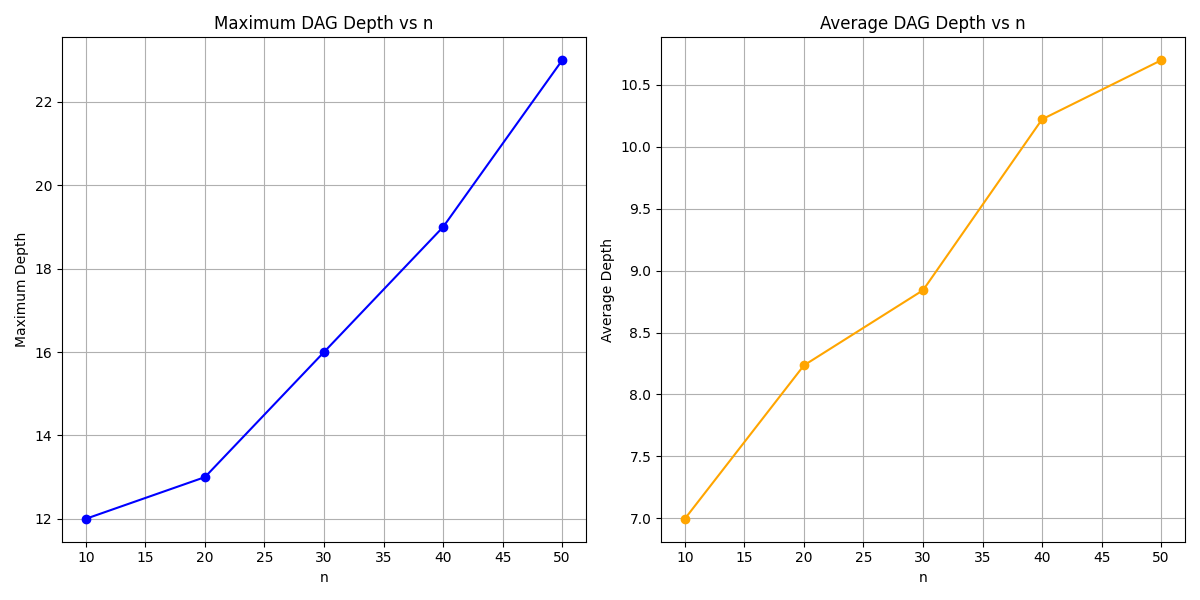
\includegraphics[width=0.9\textwidth]{Figure_1.png}
    \label{fig:model}
\end{figure*}

\hspace{0.01cm}
\\
\textbf{Short Analysis: }
\\
The result I got is reasonable, with the average depths increasing in $log n$ as expected, indicating that the algorithm effectively maintains a balanced DAG structure. 
Although the maximum depths are somewhat higher than theoretical predictions, they remain within an acceptable range considering the algorithm's randomness and the potential for local depth increases during edge legalization. 
\\
\textbf{Implementation: }
\\
The following code of randomized Delaunay triangulation algorithm with history DAG was implemented in Python:
\begin{verbatim}
# Data Structures Definitions

class Point:
    def __init__(self, x, y):
        self.x = x
        self.y = y

class SegmentWrapper:
    """
    Helper class to uniquely identify a segment irrespective of point order.
    """
    def __init__(self, p1, p2):
        # Ensure consistent ordering
        if (p1.x, p1.y) < (p2.x, p2.y):
            self.p1, self.p2 = p1, p2
        else:
            self.p1, self.p2 = p2, p1

    def __eq__(self, other):
        return (self.p1.x, self.p1.y) == (other.p1.x, other.p1.y) and \
               (self.p2.x, self.p2.y) == (other.p2.x, other.p2.y)

    def __hash__(self):
        return hash(((self.p1.x, self.p1.y), (self.p2.x, self.p2.y)))

    def __repr__(self):
        return f"Segment(({self.p1.x}, {self.p1.y}) - ({self.p2.x}, {self.p2.y}))"

class Triangle:
    def __init__(self, p1, p2, p3):
        self.vertices = [p1, p2, p3]  # Points
        self.edges = [
            SegmentWrapper(p1, p2),
            SegmentWrapper(p2, p3),
            SegmentWrapper(p3, p1)
        ]
        self.neighbors = {}  # edge -> adjacent triangle
        self.children = []  # For history DAG

    def contains_point(self, point):
        return point in self.vertices

    def __repr__(self):
        verts = ', '.join([f"({p.x}, {p.y})" for p in self.vertices])
        return f"Triangle({verts})"

class HistoryDAGNode:
    def __init__(self, triangle):
        self.triangle = triangle  # Triangle object
        self.children = []        # List of HistoryDAGNode

    def add_child(self, child_node):
        self.children.append(child_node)

# Delaunay Triangulation Class

class DelaunayTriangulation:
    def __init__(self, points):
        self.points = points  # List of Point objects
        self.segments = {}    # SegmentWrapper -> list of adjacent Triangles
        self.triangles = []   # List of Triangle objects
        self.history_root = None

    def create_super_triangle(self):
        """
        Create a super-triangle that encompasses all the points.
        """
        min_x = min(p.x for p in self.points)
        max_x = max(p.x for p in self.points)
        min_y = min(p.y for p in self.points)
        max_y = max(p.y for p in self.points)

        dx = max_x - min_x
        dy = max_y - min_y
        delta_max = max(dx, dy) * 100  # Make it large enough

        # Create three points that form a super-triangle
        p1 = Point(min_x - delta_max, min_y - delta_max)
        p2 = Point(min_x + 2 * delta_max, min_y - delta_max)
        p3 = Point(min_x - delta_max, max_y + 2 * delta_max)

        super_triangle = Triangle(p1, p2, p3)
        self.triangles.append(super_triangle)
        self.history_root = HistoryDAGNode(super_triangle)

        # Add segments of the super-triangle
        for edge in super_triangle.edges:
            self.segments.setdefault(edge, []).append(super_triangle)

    def locate_containing_triangle(self, point):
        """
        Traverse the history DAG to locate the triangle containing the point.
        """
        node = self.history_root
        while node.children:
            found = False
            for child in node.children:
                if self.point_in_triangle(point, child.triangle):
                    node = child
                    found = True
                    break
            if not found:
                break  # Point not found in any child; fallback
        # Now, node.triangle should contain the point
        return node.triangle, node

    @staticmethod
    def point_in_triangle(p, triangle):
        """
        Check if point p is inside the given triangle using barycentric coordinates.
        """
        def sign(p1, p2, p3):
            return (p1.x - p3.x) * (p2.y - p3.y) - \
                   (p2.x - p3.x) * (p1.y - p3.y)

        b1 = sign(p, triangle.vertices[0], triangle.vertices[1]) < 0.0
        b2 = sign(p, triangle.vertices[1], triangle.vertices[2]) < 0.0
        b3 = sign(p, triangle.vertices[2], triangle.vertices[0]) < 0.0

        return ((b1 == b2) and (b2 == b3))

    def insert_point(self, point):
        """
        Insert a single point into the triangulation.
        """
        containing_triangle, containing_node = self.locate_containing_triangle(point)

        # Remove the containing triangle
        self.triangles.remove(containing_triangle)

        # Create new triangles by connecting the point 
        # to the vertices of the containing triangle
        t1 = Triangle(point, containing_triangle.vertices[0], 
            containing_triangle.vertices[1])
        t2 = Triangle(point, containing_triangle.vertices[1], 
            containing_triangle.vertices[2])
        t3 = Triangle(point, containing_triangle.vertices[2], 
            containing_triangle.vertices[0])

        # Set neighbors
        self.set_neighbors(t1, containing_triangle)
        self.set_neighbors(t2, containing_triangle)
        self.set_neighbors(t3, containing_triangle)

        # Add new triangles
        self.triangles.extend([t1, t2, t3])

        # Update segments
        for t in [t1, t2, t3]:
            for edge in t.edges:
                self.segments.setdefault(edge, []).append(t)

        # Update history DAG
        child_nodes = [
            HistoryDAGNode(t1),
            HistoryDAGNode(t2),
            HistoryDAGNode(t3)
        ]
        for child in child_nodes:
            containing_node.add_child(child)

        # Edge Legalization
        for t in [t1, t2, t3]:
            for edge in t.edges:
                if point in [edge.p1, edge.p2]:
                    self.legalize_edge(edge, t, point)

    def set_neighbors(self, new_triangle, old_triangle):
        """
        Set the neighboring triangles for the new triangle.
        """
        for edge in new_triangle.edges:
            if edge in self.segments:
                for neighbor in self.segments[edge]:
                    if neighbor != old_triangle and neighbor != new_triangle:
                        new_triangle.neighbors[edge] = neighbor
                        neighbor.neighbors[edge] = new_triangle

    def legalize_edge(self, edge, triangle, point):
        """
        Legalize an edge to restore the Delaunay condition.
        """
        if edge not in triangle.neighbors:
            return  # Boundary edge

        neighbor = triangle.neighbors[edge]
        if neighbor is None:
            return

        # Find the opposite point in the neighbor triangle
        opposite_point = [v for v in neighbor.vertices 
                            if v not in [edge.p1, edge.p2]][0]

        if self.in_circumcircle(opposite_point, triangle):
            # Perform edge flip
            new_triangles = self.edge_flip(triangle, neighbor, edge, 
                                            point, opposite_point)
            for new_t in new_triangles:
                for e in new_t.edges:
                    if point in [e.p1, e.p2]:
                        self.legalize_edge(e, new_t, point)

    def edge_flip(self, t1, t2, edge, point, opposite_point):
        """
        Flip the shared edge between two triangles.
        """
        # Remove old triangles
        self.triangles.remove(t1)
        self.triangles.remove(t2)

        # Remove edge from segments
        self.segments[edge].remove(t1)
        self.segments[edge].remove(t2)
        if not self.segments[edge]:
            del self.segments[edge]

        # Create new edge
        new_edge = SegmentWrapper(point, opposite_point)

        # Create new triangles
        new_t1 = Triangle(point, edge.p1, opposite_point)
        new_t2 = Triangle(point, opposite_point, edge.p2)

        # Update segments
        for t in [new_t1, new_t2]:
            for e in t.edges:
                self.segments.setdefault(e, []).append(t)

        # Update neighbors
        self.update_neighbors_after_flip(t1, t2, new_t1, new_t2, edge, new_edge)

        # Add new triangles
        self.triangles.extend([new_t1, new_t2])

        # Update history DAG
        parent_node = HistoryDAGNode(None)
        t1_node = self.find_history_node(self.history_root, t1)
        t2_node = self.find_history_node(self.history_root, t2)
        parent_node.add_child(t1_node)
        parent_node.add_child(t2_node)
        new_t1_node = HistoryDAGNode(new_t1)
        new_t2_node = HistoryDAGNode(new_t2)
        parent_node.add_child(new_t1_node)
        parent_node.add_child(new_t2_node)

        return [new_t1, new_t2]

    def update_neighbors_after_flip(self, t1, t2, new_t1, new_t2, old_edge, new_edge):
        """
        Update neighbor relationships after an edge flip.
        """
        # Set neighbors for new_t1
        new_t1.neighbors[new_edge] = new_t2
        new_t2.neighbors[new_edge] = new_t1

        # Update other neighbors
        for e in new_t1.edges:
            if e != new_edge:
                for neighbor in self.segments[e]:
                    if neighbor != new_t1:
                        new_t1.neighbors[e] = neighbor
                        neighbor.neighbors[e] = new_t1

        for e in new_t2.edges:
            if e != new_edge:
                for neighbor in self.segments[e]:
                    if neighbor != new_t2:
                        new_t2.neighbors[e] = neighbor
                        neighbor.neighbors[e] = new_t2

    def find_history_node(self, node, triangle):
        """
        Find the history DAG node corresponding to the given triangle.
        """
        if node.triangle == triangle:
            return node
        for child in node.children:
            result = self.find_history_node(child, triangle)
            if result is not None:
                return result
        return None

    def in_circumcircle(self, point, triangle):
        """
        Check if a point is inside the circumcircle of a triangle.
        """
        ax, ay = triangle.vertices[0].x - point.x, triangle.vertices[0].y - point.y
        bx, by = triangle.vertices[1].x - point.x, triangle.vertices[1].y - point.y
        cx, cy = triangle.vertices[2].x - point.x, triangle.vertices[2].y - point.y

        det = (ax * (by * (cx**2 + cy**2) - cy * (bx**2 + by**2)) -
               ay * (bx * (cx**2 + cy**2) - cx * (bx**2 + by**2)) +
               (ax**2 + ay**2) * (bx * cy - cx * by))

        return det > 0

    def build_triangulation(self):
        """
        Build the triangulation by inserting all points.
        """
        self.create_super_triangle()
        for point in self.points:
            self.insert_point(point)
        self.remove_super_triangle()

    def remove_super_triangle(self):
        """
        Remove any triangles that share a vertex with the super-triangle.
        """
        # Super-triangle vertices
        super_vertices = set(self.history_root.triangle.vertices)
        self.triangles = [t for t in self.triangles 
                            if not any(v in super_vertices for v in t.vertices)]

    def calculate_dag_depths(self):
        """
        Calculate maximum and average depths of the history DAG.
        """
        depths = []
        queue = deque([(self.history_root, 0)])

        while queue:
            node, depth = queue.popleft()
            if not node.children:
                depths.append(depth)
            else:
                for child in node.children:
                    queue.append((child, depth + 1))

        max_depth = max(depths) if depths else 0
        avg_depth = sum(depths) / len(depths) if depths else 0
        return max_depth, avg_depth
    
    def plot_triangulation(self):
        """
        Plot the triangulation.
        """
        plt.figure(figsize=(8, 8))
        for triangle in self.triangles:
            x_coords = [vertex.x for vertex in triangle.vertices + [triangle.vertices[0]]]
            y_coords = [vertex.y for vertex in triangle.vertices + [triangle.vertices[0]]]
            plt.plot(x_coords, y_coords, 'k-')
        plt.scatter([p.x for p in self.points], 
                    [p.y for p in self.points], color='red', s=10)
        plt.axis('equal')
        plt.title('Delaunay Triangulation')
        plt.show()
\end{verbatim}


\end{document}
